We now develop interesting geometry considerations that relate to the linear optimization problem, and more precisely, to its constraints region. 

The constraints region is the subset
\[
    \{ x \in \mathbf R^n, \forall i \in \{ 1, ..., m \}, \sum_{j=1}^n a_{ij} x_j \leqslant b_i \quad \textrm{and} \quad \forall j \in \{ 1, ..., m \}, x_j \geqslant 0 \},
\]
where $ (a_{ij})_{\substack{1 \leq i \leq m \\ 1 \leq j \leq n}} $, $ (b_j)_{1 \leq j \leq n} $, $ (c_i)_{1 \leq i \leq m} $, are real numbers. Or, equivalently, it is
\[
    \{ x \in \mathbf R^n, Ax \leqslant b \quad \textrm{and} \quad x \geqslant 0 \},
\]
wher $ A \in \mathbf R^{m \times n} $ and $ b \in \mathbf R^m $.

Note that the region $ \{ x \in \mathbf R^n, x \geqslant 0 \} $ is also of the form $ \{ x \in \mathbf R^n, Ax \leqslant b \} $ with $ A = -I $ and $ b = 0 $. Thus, we may narrow our study down to that of the regions of the form.

As it turns out, these regions are convex polytopes.

\begin{theorem}\label{thm:polytopes-are-intersections-of-closed-halfspaces}
    Let $ A $ be a region of $ \mathbf R^n $. The following assertions are equivalent : 
    
    (i) $ A $ can be written as the convex hull of a finite number of points in $ \mathbf R^n $.

    (ii) $ A $ can be written as the intersection of a finite number of closed half-spaces (defined by affine hyperplanes) $ \mathbf R^n $.
\end{theorem}

This theorem is sometimes referred to as the Minkowki-Weyl theorem. But, not that often, actually. I highly suspect that neither Minkowski, nor Weil, neither have to do with the statement, nor with the proof of this theorem. 

We do not here provide a proof for this theorem, as the proof is a bit long and not very interesting in our opinion. It can be found in this bachelor thesis \cite{chappell2019}, it is also the Corollary 13.6 of Section 13.5 in Chapter 13 of the more standard reference \cite{jantosciak1979}. Though the proof requires to formally investigate (in particular, define properly) the notions of \textit{face} and \textit{vertice} of a $ n $-dimensional polytope, it appears clear to us that a small drawing is much more enlightening. Interestingly, a generalization to infinite-dimensional spaces can be found in \cite{LeRomer2023}.

\begin{definition}[Convex polytope]
    A region $ A \subset \mathbf R^n $ is a \textit{convex polytope} if it satisfies one of the equivalent conditions of Theorem~\ref{thm:polytopes-are-intersections-of-closed-halfspaces}
\end{definition}

Again, a small drawing easily convices us that the following definition is the right one.

\begin{definition}[Polytope]\label{def:polytopes}
    A \textit{polytope} is a finite union of convex polytopes.
\end{definition}

We give another interesting point of view for this definition. Recall first that polygons have ears.

\begin{definition}
    In a two-dimentional polygon, an \textit{ear} consists in two consecutive, non-parallel segments, such that the (non-flat) triangle defined by the three involved vertices is entirely contained \textit{inside} the polygon. 
\end{definition}

\begin{remark}
    Though the fact that plane simple closed curves always define an \textit{interior} and an \textit{exterior} is far from being trivial and consists in Jordan's theorem \cite{jordan1893}, the case of polygons is much easier \cite{courant1941}.
\end{remark}

\begin{example}
    In the following figure, $ MAB $ and $ DEF $ form ears, while $ GHI $, $ JKL $ and $ KLM $ do not.

    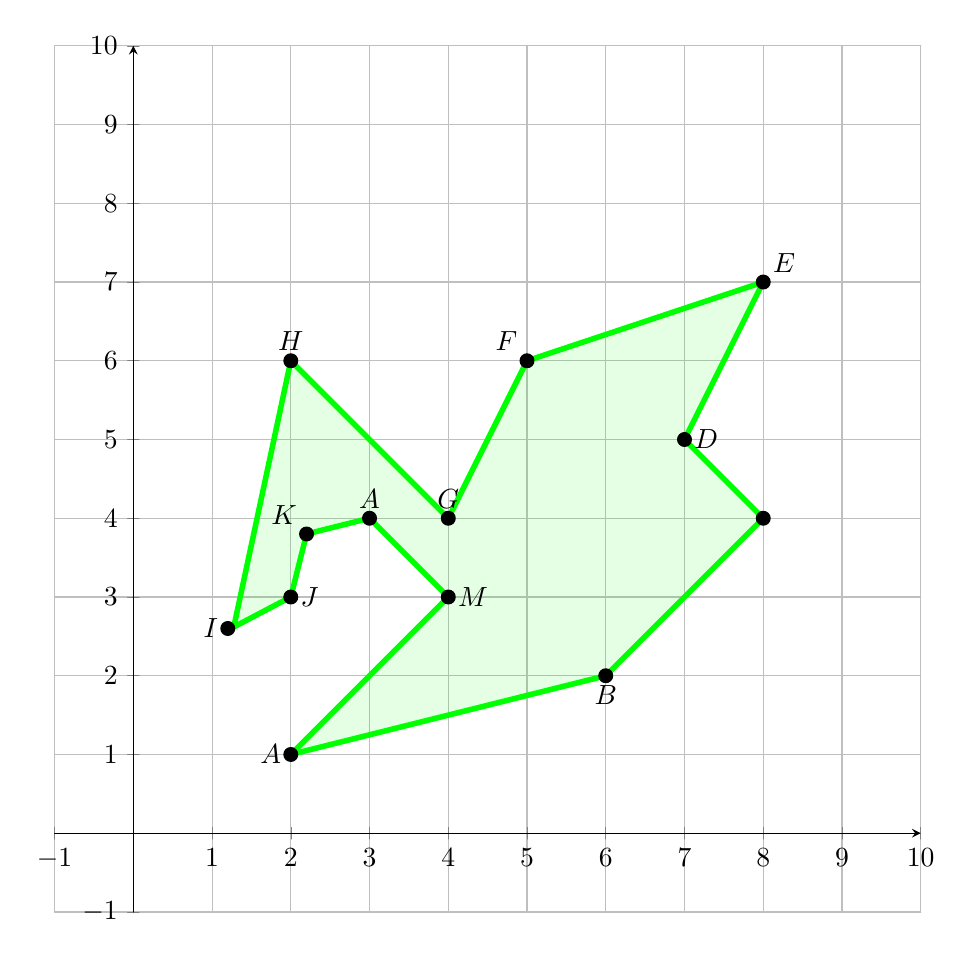
\begin{tikzpicture}[line cap=round,line join=round,x=1.0cm,y=1.0cm]
        \begin{axis}[
            x=1.0cm,y=1.0cm,
            axis lines=middle,
            ymajorgrids=true,
            xmajorgrids=true,
            xmin=-1.0,
            xmax=10.0,
            ymin=-1.0,
            ymax=10.0,
            xtick={-1.0,0.0,...,10.0},
            ytick={-1.0,0.0,...,10.0},
        ]
            \clip(-1.,-1.) rectangle (10.,8.);
            \fill[line width=2.pt,color=green,fill=green,fill opacity=0.1] (2.,1.) -- (6.,2.) -- (8.,4.) -- (7.,5.) -- (8.,7.) -- (5.,6.) -- (4.,4.) -- (2.,6.) -- (1.2759760937888327,2.6186724615855757) -- (2.,3.) -- (2.2,3.8) -- (3.,4.) -- (4.,3.) -- cycle;
            \draw [line width=2.pt,color=green] (2.,1.)-- (6.,2.);
            \draw [line width=2.pt,color=green] (6.,2.)-- (8.,4.);
            \draw [line width=2.pt,color=green] (8.,4.)-- (7.,5.);
            \draw [line width=2.pt,color=green] (7.,5.)-- (8.,7.);
            \draw [line width=2.pt,color=green] (8.,7.)-- (5.,6.);
            \draw [line width=2.pt,color=green] (5.,6.)-- (4.,4.);
            \draw [line width=2.pt,color=green] (4.,4.)-- (2.,6.);
            \draw [line width=2.pt,color=green] (2.,6.)-- (1.2759760937888327,2.6186724615855757);
            \draw [line width=2.pt,color=green] (1.2759760937888327,2.6186724615855757)-- (2.,3.);
            \draw [line width=2.pt,color=green] (2.,3.)-- (2.2,3.8);
            \draw [line width=2.pt,color=green] (2.2,3.8)-- (3.,4.);
            \draw [line width=2.pt,color=green] (3.,4.)-- (4.,3.);
            \draw [line width=2.pt,color=green] (4.,3.)-- (2.,1.);
            \begin{scriptsize}
                \draw [fill=black] (2.,1.) circle (2.5pt) node[left] {$A$};
                \draw [fill=black] (6.,2.) circle (2.5pt) node[below] {$B$};
                \draw [fill=black] (8.,4.) circle (2.5pt);
                \draw [fill=black] (7.,5.) circle (2.5pt) node[right] {$D$};
                \draw [fill=black] (8.,7.) circle (2.5pt) node[above right] {$E$};
                \draw [fill=black] (5.,6.) circle (2.5pt) node[above left] {$F$};
                \draw [fill=black] (4.,4.) circle (2.5pt) node[above] {$G$};
                \draw [fill=black] (2.,6.) circle (2.5pt) node[above] {$H$};
                \draw [fill=black] (1.2,2.6) circle (2.5pt) node[left] {$I$};
                \draw [fill=black] (2.,3.) circle (2.5pt) node[right] {$J$};
                \draw [fill=black] (2.2,3.8) circle (2.5pt) node[above left] {$K$};
                \draw [fill=black] (3.,4.) circle (2.5pt) node[above] {$A$};
                \draw [fill=black] (4.,3.) circle (2.5pt) node[right] {$M$};
            \end{scriptsize}
        \end{axis}
    \end{tikzpicture}
\end{example}

The following theorem is due to Meisters~\cite{meisters1975}.

\begin{theorem}(Polygons have ears)
    In the plane, a simple polygon has at least two ears.
\end{theorem}

\begin{remark}
    It yields a simple algorithm for finding a triangulation of a polygon in the plane : find an ear, remove it, and iterate ! Whereas the algorithm is simple, its complexity of such algorithm is sub-optimal, as shown in \cite{chazelle1991} : B. Chazelle provided a linear algorithm, but much more complex.
\end{remark}

\begin{remark}
    This little detour in polygon triangulations, to explain two things. First, that polygon triangulations exist (and above is explained how to find them)---they are very useful when dealing with polygons in geometry. Second, we can now re-interpret Definition~\ref{def:polytopes} in light of this fact : recall that triangles are two-dimentional simplexes, i.e., they are always convex regions of the plane. Therefore, since the existence of polygon triangulations implies they can always be written as a union of triangles, (non-convex) polygons are unions of convex regions. So, in this perspective, the definition of a non-convex polygon is the right generalization of that of a polygon to $ n $ dimensions !
\end{remark}

Let's get back to the link with linear optimization.

\begin{theorem}
    Let $ A \in \mathbf R^{m \times n} $ and $ b \in \mathbf R^m $.

    Then, the region
    \[
        \{ x \in \mathbf R^n, Ax \leqslant b \}
    \]
    is a convex polytope.
\end{theorem}

\begin{proof}
    Writing the matrix product, the condition $ Ax \leqslant b $ is equivalent to
    \[
        \forall i \in \{ 1, ..., m \}, \sum_{j=1}^n a_{ij} x_j \leqslant b_i,
    \]
    but, for each $ i \in \{ 1, ..., m \} $,
    \[
        H_i^{A,b} := \{ x \in \mathbf R^n, \sum_{j=1}^n a_{ij} x_j \leqslant b_i \} 
    \]
    is clearly, by definition, an affine half-space (defined by the affine hyperplane with equation $ \sum\limits _{j=1}^na_{ij} x_j \leqslant b_i $).

    Clearly, we have
    \[
        Ax \leqslant b \iff x \in \bigcap_{i=1}^m H_i^{A,b}
    \]
    when the result, given Theorem \ref{thm:polytopes-are-intersections-of-closed-halfspaces}.

    The fact that it is convex comes from the fact that any intersection of convex regions remains convex, or by the fact that Theorem~\ref{thm:polytopes-are-intersections-of-closed-halfspaces} implies that the condition is equivalent to being a convex hull (which, needless to say, are convex).
\end{proof}

\begin{remark}
    We have written all of these developments because we find the fact that the region $ Ax \leqslant b $ is a convex polytope a very interesting one !

    It is very a well-known, very classical, and yet very interesting result, that affine hyperplanes are the regions of the form $ Ax = b $. Hence, what the regions $ Ax \leqslant b $ look like is just as interesting!
\end{remark}

\begin{proposition}
    The constraints region of a linear optimization problem, namely,
    \[
        \{ x \in \mathbf R^n, Ax \leqslant b \quad \textrm{and} \quad x \geqslant 0 \}
    \]
    is a convex polytope.
\end{proposition}

\begin{proof}
    This region is the intersection of the half-spaces defined by
    \[
        \{ x \in \mathbf R^n, \sum_{j=1}^n a_{ij} x_j \leqslant b_i \}
    \]
    for $ i \in \{ 1,...,m \} $, and the half-spaces
    \[
        \{ x \in \mathbf R^n, x_i \geqslant 0 \}
    \]
    for $ i \in \{ 1,...,m \} $.

    As a result, it is a polytope according to Theorem~\ref{thm:polytopes-are-intersections-of-closed-halfspaces}.
\end{proof}

\begin{example}
    Consider a linear optimization problem, the constraints region of which is given by :

    \[
        \left\{
            \begin{array}{l}
            x + y \geqslant 13 \\
            x - y \leqslant 5 \\
            -2x + y \leqslant 4 \\
            3x + 4y \leqslant 92 \\
            y \leqslant 14
            \end{array}
        \right.
    \]
    
    Then, this constraint region is illustrated by the following drawing.
    \begin{center}
        \begin{tikzpicture}
            \begin{axis}[
                x=0.3cm,y=0.3cm,
                axis lines=middle,
                xmin=-4.0,
                xmax=40.0,
                ymin=-3.0,
                ymax=23.0,
                xtick={-4.0,-2.0,...,40.0},
                ytick={-2.0,0.0,...,22.0},
            ]
                \clip(-4.,-3.) rectangle (40.,23.);
                \fill[line width=8.pt,color=red,fill=red,pattern=north east lines,pattern color=red] (3.,10.) -- (5.,14.) -- (12.,14.) -- (16.,11.) -- (9.,4.) -- cycle;
                \draw [line width=1.pt,domain=-12.:40.] plot(\x,{(--13.-1.*\x)/1.});
                \draw [line width=1.pt,domain=-12.:40.] plot(\x,{(--5.-1.*\x)/-1.});
                \draw [line width=1.pt,domain=-12.:40.] plot(\x,{(--4.--2.*\x)/1.});
                \draw [line width=1.pt,domain=-12.:40.] plot(\x,{(--92.-3.*\x)/4.});
                \draw [line width=1.pt,domain=-12.:40.] plot(\x,{(--14.-0.*\x)/1.});
                \begin{scriptsize}
                    \draw [fill=black] (-1.,14.) circle (2.5pt);
                    \draw [fill=black] (3.,10.) circle (2.5pt);
                    \draw [fill=black] (5.,14.) circle (2.5pt);
                    \draw [fill=black] (6.909090909090909,17.818181818181817) circle (2.5pt);
                    \draw [fill=black] (12.,14.) circle (2.5pt);
                    \draw [fill=black] (19.,14.) circle (2.5pt);
                    \draw [fill=black] (16.,11.) circle (2.5pt);
                    \draw [fill=black] (9.,4.) circle (2.5pt);
                    \draw [fill=black] (-2.,0.) circle (2.5pt);
                    \draw [fill=black] (-2.,0.) circle (2.5pt);
                    \draw [fill=black] (0.,0.) circle (2.5pt);
                    \draw [fill=black] (0.,4.) circle (2.5pt);
                    \draw [fill=black] (5.,0.) circle (2.5pt);
                    \draw [fill=black] (13.,0.) circle (2.5pt);
                    \draw [fill=black] (30.666666666666668,0.) circle (2.5pt);
                \end{scriptsize}
            \end{axis}
        \end{tikzpicture}
    \end{center}
\end{example}

To conclude, let us mention the following precision. The next section is devoted to presenting Dantzig's Simplex algorithm, more often referred to as \og The Simplex Algorithm \fg. 

\begin{definition}[Simplex]
    In a $ n $-dimensional vector (or affine) space $ E $, a \textit{simplex} is a region that can be written as the convex hull of a $ n + 1 $ points of $ E $.
\end{definition}

So the question that arises now is : what is the link between the Simplex algoritm and simplexes ? The answer is : there is none. As opposed to what its name suggests, this algorithm does not perform on a simplex. ...Unless the constraints polytope happens to be a simplex. Which is by no means always the case !